In this section, we compare two methods for performing plane-wave decomposition:
\begin{enumerate}
\item beamforming, as given by \eqnref{eq:02_Acoustical_Theory:A2mu}, and
\item pseudoinversion, as given by \eqnref{eq:02_Acoustical_Theory:A2mu_Pinv}.
\end{enumerate}
In particular, we explore the performance of each method across a range plane-wave grid densities and input ambisonics orders, $L_\text{in}$.
For all plane-wave expansions, we compute $Q$ plane-wave terms arranged on Fliege nodes and use the corresponding quadrature weights (available online).\citefooturl{FliegeNodesURL}
Additionally, for ease of comparison with $L_\text{in}$, we define the ``order'' of a given plane-wave expansion as $\sqrt{Q} - 1$.
As mentioned in \secref{sec:06_Simulation_Framework:Metrics}, all errors are computed averaging over all source azimuths and over all listener positions in the navigable region (see \figref{fig:06_Simulation_Framework:Point_Geometry}).
For these simulations, we examine a typical far-field scenario by choosing $u = 0.25$~m and $s_0 = 2.5$~m (so $\gamma = 10$).

%\subsection{Results}
In \figreftwo{fig:07_Characterization_Extrapolation:Level_Order:PWT-bf}{fig:07_Characterization_Extrapolation:Level_Order:PWT-pinv}, we plot the level errors (as defined in \secref{sec:04_Auditory_Models:Audible_Energy}) for each plane-wave decomposition method as a function of $Q$ and $L_\text{in}$.
From \figref{fig:07_Characterization_Extrapolation:Level_Order:PWT-bf}, we note a region of small errors that follows the diagonal line $L_\text{in} \approx \sqrt{Q} - 1$.
This suggests that, for the beamforming method, it is advantageous to match the number of plane-wave terms to the number of ambisonics signals, i.e., $Q \approx N_\text{in}$.
Following \citet{HahnSpors2015b}, we refer to this condition as the ``critically-sampled'' condition, since $Q = N_\text{in}$, while we refer to $Q > N_\text{in}$ as oversampled and $Q < N_\text{in}$ as undersampled.

\begin{figure*}[t]
    	\centering
    	\begin{subfigure}[b]{0.49\textwidth}
        		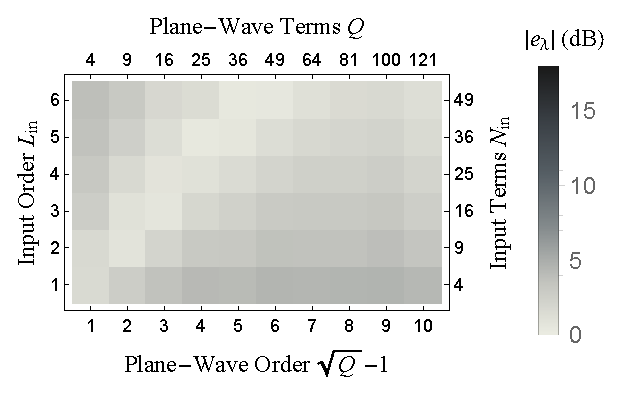
\includegraphics[width=\textwidth]{07_characterization_extrapolation/figures/audibleEnergy_order_pwt-bf.eps}
        		\caption{Level error $e_\lambda$ -- beamforming}
        		\label{fig:07_Characterization_Extrapolation:Level_Order:PWT-bf}
    	\end{subfigure}
	\hfill
    	\begin{subfigure}[b]{0.49\textwidth}
        		\includegraphics[width=\textwidth]{07_characterization_extrapolation/figures/audibleEnergy_order_pwt-pinv.eps}
        		\caption{Level error $e_\lambda$  -- pseudoinversion}
        		\label{fig:07_Characterization_Extrapolation:Level_Order:PWT-pinv}
    	\end{subfigure}
	
	\vspace{0.5cm}
	\begin{subfigure}[b]{0.49\textwidth}
        		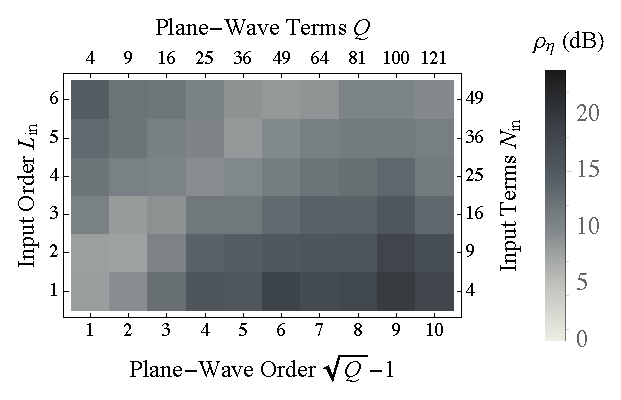
\includegraphics[width=\textwidth]{07_characterization_extrapolation/figures/scharer2009_order_pwt-bf.eps}
        		\caption{Spectral error $\rho_\eta$ -- beamforming}
        		\label{fig:07_Characterization_Extrapolation:Spectral_Order:PWT-bf}
    	\end{subfigure}
	\hfill
    	\begin{subfigure}[b]{0.49\textwidth}
        		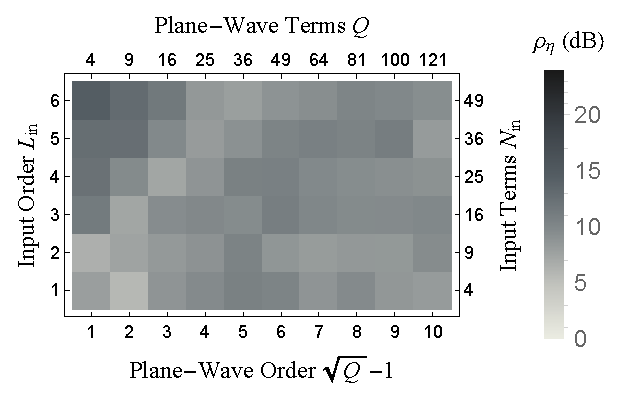
\includegraphics[width=\textwidth]{07_characterization_extrapolation/figures/scharer2009_order_pwt-pinv.eps}
        		\caption{Spectral error $\rho_\eta$ -- pseudoinversion}
        		\label{fig:07_Characterization_Extrapolation:Spectral_Order:PWT-pinv}
    	\end{subfigure}
	
	\caption[Dependence of errors on plane-wave terms and ambisonics input order.]{
	Dependence of errors on $Q$ and ambisonics input order $L_\text{in}$ (continued on p.~\pageref{fig:07_Characterization_Extrapolation:PWT_Order_Dependence:contd}).}
	\label{fig:07_Characterization_Extrapolation:PWT_Order_Dependence}
\end{figure*}

From \figref{fig:07_Characterization_Extrapolation:Level_Order:PWT-pinv}, we see a similar region of small errors, but it is less pronounced, since for $Q > N_\text{in}$ (bottom right corner of the plot), the errors are also small.
However, we note that a region of very large errors exists where $Q < N_\text{in}$ (top left corner).
This suggests that, for the pseudoinversion method, it is advantageous to have $Q \geq N_\text{in}$;
i.e., to have at least as many plane-wave terms as ambisonics signals.

The spectral errors (as defined in \secref{sec:04_Auditory_Models:Coloration_Metrics:ABSE}) for each method are plotted in \figreftwo{fig:07_Characterization_Extrapolation:Spectral_Order:PWT-bf}{fig:07_Characterization_Extrapolation:Spectral_Order:PWT-pinv}, which show trends similar to those exhibited by the level errors discussed above.
From these plots, it is clear that only the critically-sampled condition is ideal for the beamforming method.
This is in agreement with the finding of \citet[cf.~Fig.~7]{HahnSpors2015b}: that the critical-sampling condition yields decreased coloration (compared to oversampling) when using the beamforming method.
From \figref{fig:07_Characterization_Extrapolation:Spectral_Order:PWT-pinv}, we see that both the critical-sampling and oversampling conditions yield small errors for the pseudoinversion method.
Oversampling and undersampling for the beamforming method, as well as undersampling for the pseudoinversion method, all yield significantly larger errors than other conditions.

From \figreftwo{fig:07_Characterization_Extrapolation:Localization_Order:PWT-bf}{fig:07_Characterization_Extrapolation:Localization_Order:PWT-pinv}, we see that both methods yield large localization errors (as computed with \eqnref{eq:04_Auditory_Models:Localization_Error} for the localization model described in \secref{sec:05_Proposed_Models:Localization_Model}) for undersampled conditions.
For the beamforming method, the errors are otherwise uniformly small, except at very small ambisonics orders ($L_\text{in} = 1$).
That these errors do not improve with increasing $Q$ corroborates the finding of \citet[cf.~Fig.~4]{Winter2014}: that increasing the number of plane-waves beyond critically-sampled does not improve localization when using the beamforming method.
From \figref{fig:07_Characterization_Extrapolation:Localization_Order:PWT-pinv}, we see that the pseudoinversion method appears sensitive to mismatches between $Q$ and $N_\text{in}$ given the presence of large, sporadic errors that do not follow any obvious pattern.

\begin{figure*}[t]\ContinuedFloat
	\begin{subfigure}[b]{0.49\textwidth}
        		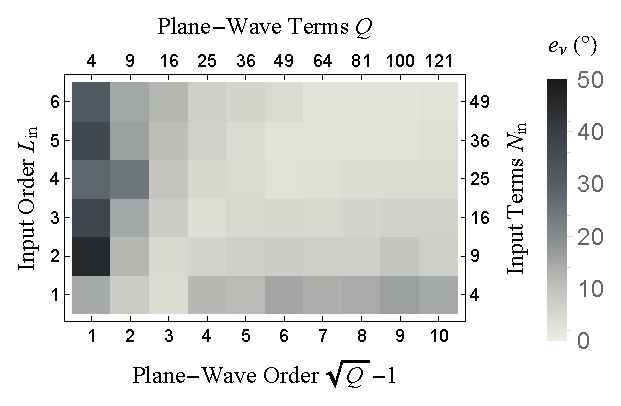
\includegraphics[width=\textwidth]{07_characterization_extrapolation/figures/tylka2017_order_pwt-bf.eps}
        		\caption{Localization error $e_\nu$ -- beamforming}
        		\label{fig:07_Characterization_Extrapolation:Localization_Order:PWT-bf}
    	\end{subfigure}
	\hfill
    	\begin{subfigure}[b]{0.49\textwidth}
        		\includegraphics[width=\textwidth]{07_characterization_extrapolation/figures/tylka2017_order_pwt-pinv.eps}
        		\caption{Localization error $e_\nu$ -- pseudoinversion}
        		\label{fig:07_Characterization_Extrapolation:Localization_Order:PWT-pinv}
    	\end{subfigure}
	
	\vspace{0.5cm}
	\begin{subfigure}[b]{0.49\textwidth}
        		\includegraphics[width=\textwidth]{07_characterization_extrapolation/figures/merimaa2005_d_order_pwt-bf.eps}
        		\caption{Diffuseness error $e_\Psi$ -- beamforming}
        		\label{fig:07_Characterization_Extrapolation:Diffuseness_Order:PWT-bf}
    	\end{subfigure}
	\hfill
    	\begin{subfigure}[b]{0.49\textwidth}
        		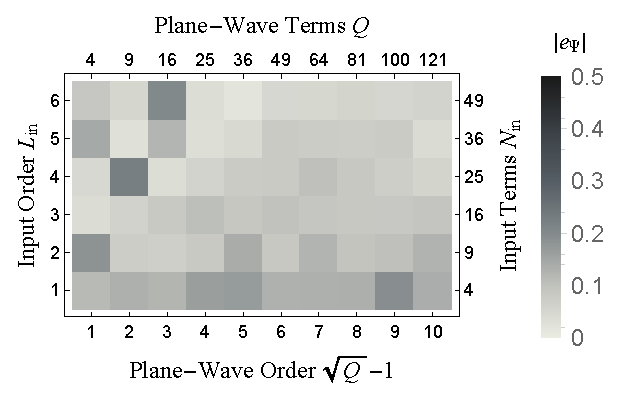
\includegraphics[width=\textwidth]{07_characterization_extrapolation/figures/merimaa2005_d_order_pwt-pinv.eps}
        		\caption{Diffuseness error $e_\Psi$ -- pseudoinversion}
        		\label{fig:07_Characterization_Extrapolation:Diffuseness_Order:PWT-pinv}
    	\end{subfigure}
	
    	\caption[]{Dependence of errors on $Q$ and ambisonics input order $L_\text{in}$ (continued from p.~\pageref{fig:07_Characterization_Extrapolation:PWT_Order_Dependence}).}
    	\label{fig:07_Characterization_Extrapolation:PWT_Order_Dependence:contd}
\end{figure*}

From the diffuseness errors (see \secref{sec:04_Auditory_Models:Diffuseness_Parameter}) plotted in \figref{fig:07_Characterization_Extrapolation:Diffuseness_Order:PWT-bf}, we see that the beamforming method only yields relatively large errors at low ambisonics orders, e.g., $L_\text{in} = 1,2$.
For the pseudoinversion method, however, we again see a sensitivity to mismatched sampling conditions, yielding relatively large errors without any discernible pattern.
Consequently, unless the plane-wave terms can be carefully chosen ahead of time for a given ambisonics order, beamforming is likely the safer method.